%---------------------------------------------------------------------
%                          Capítulo 2
%---------------------------------------------------------------------

\chapter{Marco teórico}
%---------------------------------------------------------------------
%                          Antecedentes
%---------------------------------------------------------------------

\section{Antecedentes de la Investigación}

\subsection{Antecedentes Nacionales}

\cite{jrodriguez} publico el articulo denominado ``\emph{Beneficios del modelo As a
service en las pymes}'' cuyo objetivo fue realizar una revisión de conceptos
basicos de la computación en la nube en especial de los modelos de despliegue
o modelos \emph{As a Service} y algunas consideraciones para su adopción, ventajas
y desventajas llegando a concluir que la computación en la nube puede ser una
convincente y atractiva forma de adquirir capacidades y reducir los costos; sin
embargo, la pequeña y mediana empresa necesita acercarse a las implementaciones
en la nube con los ojos abiertos y ser sensibles a algunas cuestiones clave para
asegurar que los beneficios esperados se concreten, las que se presentan a
continuación:
\begin{enumerate}[a.]
    \item Integración de las prioridades del negocio y las prioridades de las
          tecnologías de información con la estrategia de despliegue de la
          nube, es decir, los objetivos estratégicos de la empresa o de la
          unidad de negocio necesitan estar claros y entendidos, y a su vez ser
          soportados por la tecnología.
    \item Maximización en la flexibilidad y agilidad de los negocios
          relacionados con la computación en nube para un impacto máximo.
          El beneficio real de la cloud computing es su papel potencialmente
          transformador, proporcionando acceso a los recursos consistentes en
          toda la organización, con certeza y en forma oportuna.
    \item Disponibilidad 24x7, y crecimiento de la solución desplegada gracias
          a la alta escalabilidad en el modelo.
    \item La integración de los recursos de la nube y lo existente fuera de
          ella es a largo plazo; con ello se busca que las empresas puedan agilizar
          sus procesos vitales y de negocio a través del soporte tecnológico,
          lo cual a la vez le dará una ventaja competitiva. Con el tiempo, sin
          embargo, las pequeñas empresas deberían anticipar y alentar este
          desarrollo para el aprovechamiento de los recursos locales y la maximización
          de beneficios dirigidos al crecimiento de su negocio.
\end{enumerate}

El articulo en mención servirá como guía para la difusión de estas herramientas
y sus ventajas a los empresarios, así como usar los criterios de selección
sugeridos para determinar las herramientas de computación en la nube más
adecuadas.

\cite{jcampos} desarrollo el trabajo denominado ``\emph{INFORMáTICA EN LA NUBE
COMO ALTERNATIVA DE ACCESO A LA TECNOLOGíA POR PARTE DE LA PEQUEñA EMPRESA
OLN S.A}.'', cuyo objetivo fue incrementar la productividad del proceso de
administración de estados de cuenta de naves, del proceso de venta de fletes
marítimos, y del proceso de gestión de TI a través de la implementación
de los servicios informáticos en la nube en la empresa OLN, para ello utilizo
entrevistas con los gerentes así como con ciertos colaboradores, también recurrió
a los archivos del área contable para recabar datos relacionados a costos de
servicios y productos, también se revisaron los contratos de servicio que fueran
pertinentes para el estudio. Otra de las fuentes de información estuvo constituida
por las bitácoras electrónicas y reportes tanto de las aplicaciones especializadas de
TI, de los softwares elaborados adhoc para determinados procesos y de las aplicaciones en la nube
Se recurrió además a la observación directa de las instalaciones, equipos y de las personas
dentro de su quehacer cotidiano. La técnica de medición que se empleó fue por escala de
razón y para el análisis de los datos se utilizó dos enfoques, descriptivo e inferencial.
En cuanto al análisis descriptivo se emplearon medidas de tendencia central tales como
la media aritmética (promedio) y moda (la que más se repite) También se utilizó la
desviación estándar, curtosis y la asimetría.
En lo relacionado a medidas de variabilidad se empleó la desviación estándar habiéndose
realizado con anterioridad el análisis de la dispersión de los datos mediante gráficos.
La distribución de los datos está conforme con los supuestos de la normalidad
En relación a los enfoques inferenciales se comprobó la normalidad de los datos y se
verificó que eran paramétricos razón por la cual se empleó la T-Student por medio del
software estadístico SPSS.

En dicho trabajo llego muchas conclusiones, algunas de las cuales fueron:
\begin{enumerate}[a.]
    \item La adopción del modelo en la nube suscita muchas dudas, aunque es en
          los años recientes en que ha alcanzado niveles cada vez más amplios
          de difusión y también de oferta de servicios, sin embargo vencer la
          resistencia de las pequeñas empresas como OLN para embarcarse en un
          aventura tecnológica en la cual la desmaterialización de la
          infraestructura juega un papel preponderante fue una tarea difícil
          de asumir, primero porque no se tienen a la vista los componentes
          tangibles que albergan los valiosos activos de información de la
          empresa y por otro lado porque tampoco se sabe en qué parte del
          planeta estos se encuentran, esto crea una sensación de desamparo en
          la plana directiva de lo empresa lo cual fue necesario vencer
          pacientemente abogando por el elemento primario que siempre está en
          las consideraciones del propietario y/o gerente de una empresa y esto
          es el aspecto económico.
    \item Es así que OLN dio el primer paso, tímido al principio, de arriesgarse
          a ahondar en el modelo en la nube y del autor de esta tesis de acompañarlos
          en la aventura de mostrarles que el modelo en la nube es mucho más
          que una alternativa barata de tercerización de servicios. Lo dicho
          anteriormente llevó a que el proyecto se extendiera al conjunto de
          los procesos de la empresa y se viera de que forma el nuevo modelo
          podía incrementar la productividad puntual de los procesos, vistos
          estos de manera ecléctica.
    \item De la idea establecida en la mente de los directivos de OLN en la cual
          toda automatización de procesos deía hacerse a la medida con la
          consecuente contratación de especialistas, equipos, licencias, etc.
          o de lo contrario con la compra de un software ya echo y que debía
          pasar por un doloroso proceso de personalización con la compra también
          de licencias, eventualmente de equipos y siempre con la participación
          de expertos en informática, se pasó de pronto al empleo de aplicaciones
          en la nube listas para ser usadas desde el primer momento y que inclusive
          podían ser buscadas y encontradas en Internet con la ayuda de los
          mismos interesados sin que mediara \emph{un equipo de expertos de TI},
          con la posibilidad además de usar un periodo de prueba gratuito,
          usualmente de un mes, otorgado por los proveedores
    \item De este modo se alcanzó el primer objetivo primario que tenía que
          ver con el aumento de la productividad y que en el caso presente se
          consiguió al elevar la productividad del proceso de administración
          de estados de cuentas de naves elevando la media de estados de cuenta
          procesados por hora hombre de 0.58 a 0.65, sin contar con los beneficios
          intangibles que conlleva el haber aumentado la satisfacción de los
          clientes a los cuales se les brindada este servicio y la aligeración
          de la carga operativa del personal encargado de esta tarea
    \item El aumento de la productividad también se reflejó en las ventas de
          fletes marítimos en cuyo caso fue necesario gestionar los cambios en
          el proceso de ventas de manera más \emph{fina} en la medida que el personal
          de ventas, bajo el esquema anterior a la adopción del modelo en la
          nube, operaba cada uno como un compartimento estanco en donde cada
          integrante del equipo de ventas tenía sus clientes (no de la empresa
          sino que los consideraban suyos a título personal de modo que si se
          iban de la empresa se llevaban a sus clientes ) y operaba de manera
          más o menos independiente. Vencida la resistencia al cambio, entre
          otras cosas, con la incorporación intencional del gerente de ventas
          al equipo del proyecto de modo que este actuara además como catalizador
          de las reacciones de sus subordinados y del apoyo explícito al
          proyecto manifestado personalmente por el gerente general y propietario
          de la empresa.
    \item Se automatizó la administración del proceso de ventas de fletes y
          como consecuencia se obtuvo un incremento en las ventas de 12\% con
          respecto al periodo anterior. Nuevamente en este caso la manifestación
          tangible de beneficio se da por el porcentaje de incremento en las ventas,
          sin embargo se obtuvieron otros beneficios menos evidentes como la
          recolección de métricas diversas sobre todo el proceso de ventas,
          la centralización de la información de los clientes, de modo que
          estos dejaron de ser propiedad de los representantes comerciales para
          pasar a ser clientes de la empresa, la disponibilidad de múltiples
          análisis provistos de manera automática por la aplicación y algo
          muy importante, la adopción de las mejores prácticas para el proceso
          de ventas las cuales vienen ya incorporadas en la solución adoptada.
    \item En un nivel más bajo de la adopción del modelo en la nube que es
          el que corresponde a la infraestructura como servicio (IaaS) y la
          plataforma como servicio (PaaS) también se obtuvieron beneficios
          relevantes, de carácter económico en primer lugar pero también
          al nivel operativo puesto el proceso de atención de las necesidades
          de especializadas de TI pasó de ser básicamente presencial a
          mayoritariamente remoto además de reducir drásticamente el empleo
          de ciertos especialistas y de simplificar tremendamente la administración
          de TI y liberando el espacio físico que otrora fuera ocupado por la
          infraestructura de TI.
    \item Lo anterior tiene que ver con el segundo objetivo secundario de este
          trabajo que consistió en aumentar la productividad del proceso de
          gestión de TI con respecto al costo de adquisición lo cual dio como
          resultado que bajo el modelo convencional se procesaron 31.60 transacciones
          por cada dólar invertido durante el periodo pre test, mientras que
          bajo el modelo en la nube la cantidad de transacciones por dólar
          aumenta a 348.54 es decir el costo por transacción durante el post
          test es 1,003\% más bajo que el pretest.
    \item En lo referente a la productividad de TI con respecto a las horas
          hombre de soporte se ha arribado a un resultado positivo al corroborarse
          que en el que en el periodo pre-test se empleaba una hora hombre por
          cada 479 transacciones realizadas, mientras que en post test este valor
          ascendió a 1,101 transacciones por hora hombre empleada en dar
          mantenimiento a TI, lo cual verifica que el incremento del post test
          fue de 130\% con respecto al pre test.
    \item Se ha mencionado anteriormente que la infraestructura de TI fue llevada
          a la nube lo cual comportó un ahorro fundamentalmente económico,
          pero existe otra faceta, nuevamente difícil de medir, pero que tiene
          un potencial muy grande, esto es que en el esquema tradicional la
          capacidad de TI estaba constreñida a las limitaciones físicas de los
          equipos que poseía la empresa y cualquier ampliación resultaba
          costosa en tiempo y dinero, mientras que bajo el modelo en la nube
          los límites han desaparecido, la capacidad de procesamiento de OLN
          se ha tornado virtualmente infinita y aun así sin que se tenga que
          incurrir en grandes inversiones y esperas.
    \item Lo dicho en el párrafo anterior a potenciado las posibilidades de OLN
          puesto que puede responder a exigencias en cuanto a sofisticación
          tecnológica de ciertos clientes transnacionales, lo cual lo pone en
          posición de competir con empresas de mucha mayor envergadura sin
          contar con que ahora cuenta con los recursos para montar una infraestructura
          de TI compleja para probar o demostrar algún producto o servicio (esto
          se da por ejemplo cuando se participa en una licitación en donde se
          debe estar en capacidad de operar algún proceso automatizado poco
          después de haber ganado la buena pro) y luego desmontarla rápidamente
          con poca esfuerzo y sin inversiones de capital.
\end{enumerate}

El trabajo mencionado servirá como referencia para la elaboración de los instrumentos
de medición ya que se trata de un caso muy similar al presente trabajo pero limitado
a una sola empresa.

%-----------------
\subsection{Antecedentes Internacionales}

\cite{ercolani} publico el articulo denominado ``\emph{Análisis del potencial del
Cloud Computing para las PYMEs.}'' con el objetivo de análizar la computación en nube
para la pequeña y mediana empresas (PYMEs) como una solución de las cuestiones relativas a la
introducción o la evaluación de las nuevas tecnologéas que pueden beneficiar a la empresa.
Con este fin se crea un \emph{índice de Potencial de Adopción} (IPA) que tiene
como objetivo facilitar el proceso de evaluación y comparación a la adopción de
esta tecnología evaluando: los requisitos funcionales, el costo total de propiedad,
las preocupaciones y beneficios conexos.
En este artículo se desarrolla un modelo integrado, en tres etapas, útil para
orientar la evaluación de un genérico \emph{software como servicio} (SaaS) en nube
pública, ofreciendo al mismo tiempo, una visión derivada de la literatura científica.
El resultado del proceso de análisis expuesto genera el IPA (numero valorado
entre 1 y 4) que indica el nivel de utilidad para la empresa a la adopción del
software SaaS analizado. En dicho trabajo se llego a las siguientes conclusiones:
\begin{enumerate}[a.]
    \item En este articulo se presenta un método integrado por el cálculo de un
          índice que indica el potencial de adopción de un genérico programa SaaS
          en nube publica por parte de una pequeña o mediana empresa.
    \item El índice IPA quiere facilitar, en particular las PYMEs españolas, a
          considerar la opción de SaaS, como CRM o ERP, en entorno cloud computing
          a niveles comparables a las grandes empresas porque estudios aprecian que el
          tamaño no es un factor determinante de la adopción de las TIC, pero es
          dominante el conocimiento en TIC de los propietarios y la actitud hacia
          el crecimiento (Levy et al., 2001).
    \item Para la elaboración del IPA se analiza el modelo de implementación en
          nube publica ya que:
          \begin{itemize}
              \item Las PYMEs no se inclinan hacia las inversiones de capital
                    significativas en hardware y software;
              \item No tienen los conjuntos de habilidades necesarias para implementar
                    complejas soluciones TIC;
              \item Para la PYMEs que no poseen un departamento IT o instalaciones
                    propias la adopción de SaaS en la nube publica no requiere
                    inversiones en infraestructura y al mismo tiempo permite un nivel de
                    escalabilidad sin precedentes.
          \end{itemize}
      \item Las soluciones SaaS en la nube publica ayudan a las PYMEs en la
            reducción de las inversiones iniciales en TIC permitiendo de llegar
            rápidamente hacia el mercado (time to market) y consecuentemente a
            ser más productiva, más competitiva y más rentable.
      \item Varios proveedores ofrecen soluciones SaaS que puede ser rápidamente
            adoptadas por las PYMEs a un bajo costo o por lo menos que se puede
            calcular por adelantado con buena aproximación, utilizando metodologías
            conocidas (como el TCO o el ROI).
      \item La introducción de la tecnología de cloud no es una medida fácil y
            normalmente quien decide en las PYMEs no tiene todos los conocimientos
            necesarios. Por eso la elaboración del IPA y su metodología pueden
            ser a la vez más completa y concisa de la sola evaluación económica.
      \item La novedad del modelo integrado presentado es incluir y apreciar la
            mayor parte de las características destacadas por el modelo de cloud
            computing y permitir la evaluación de su importancia con referencia
            de las características específicas y la forma en que se resume esta
            función en la solución de software SaaS examinado.
      \item El IPA, tratando de no ser el sólo apoyo a las decisiones, puede ser
            utilizado por las personas en cargo por la evaluación o comparación de
            soluciones SaaS a implementar en la empresa con agilidad adecuada y
            dando la oportunidad de profundizar el significado del número único
            por la descomposición en varios factores que han generado.
\end{enumerate}

El trabajo en menciín servira para adoptar el IPA a nuestro caso de estudio para
determinar el grado de utilidad de las herramientas de computación en la nube
en la gestión de las MiPYMEs pertenecientes al Centro de Desarrollo Empresarial
del Cusco.

\cite{diaz} desarrolló el trabajo ``\emph{EL CLOUD COMPUTING EN LA PYME ESPAñOLA}''
con el objetivo de analizar las posibilidades de uno de los productos de la empresa
Intelligence Partner, que consiste en una aplicación de gestión de activos inmobiliarios, y
para ello se puso en contexto el entorno de las Pymes y más en concreto el
sector inmobiliario español con la intención de ver las posibilidades de venta
que tiene esta aplicación en la nube, llegando a concluir que a pesar beneficios
destacados a lo largo de todo el documento, el cloud computing es una tecnología
relativamente nueva. Hay varias cuestiones que deben tenerse en cuenta antes cambiar
todos los sistemas tradicionales de la pequeña empresa por la computación en la nube.
A continuación presentamos algunos aspectos que deben considerarse antes de que una
empresa decida adaptar sus sistemas a la nube:
\begin{enumerate}[a.]
    \item   Es importante tener un profundo conocimiento de la infraestructura de TI
            existente. Se recomienda a las empresas tener en cuenta cuatro puntos
            antes de tomar una decisión, el tamaño de las infraestructuras de TI, los
            patrones de uso, la sensibilidad de los datos y lo importante que son las
            operaciones informáticas para la empresa.
    \item   Muchos analistas han señalado el problema del monopolio a la hora de
            ofrecer servicios de cloud computing. La cuestión de la dependencia de
            un proveedor puede tener graves repercusiones para las pequeñas
            empresas en caso de pérdida de datos. A medida que los servicios se
            ofrecen a través de software propietario y la falta de normas hace de la
            portabilidad de una de las principales preocupaciones.
    \item   Se espera que la nube maneje una gran cantidad de datos. Por lo tanto,
            es importante entender las cuestiones clave en cuanto a la seguridad y
            los riesgos potenciales. La revisión de los protocolos de seguridad en
            varios modelos de cloud revela la necesidad de un marco estandarizado.
            Por ejemplo, con SaaS, una de las principales preocupaciones es la falta
            de control y la total dependencia del proveedor para garantizar las
            medidas de seguridad adecuadas. Otra cuestión es garantizar la
            seguridad, la integridad y la persistencia de los datos durante la
            transferencia de datos dentro y el mantenimiento de la confidencialidad
            de los datos de los clientes
\end{enumerate}

El mencionado trabajo servirá para elaborar el diseño operativo concreto para la
implementación de cada herramienta en las MiPYME del Centro de Desarrollo
Empresarial del Cusco ya que se trata de un caso de estudio de implementación

\section{Bases Teóricas}

\subsection{Computación en la nube}

\subsubsection{Definición de Computación en la nube}
Según \cite{nist} definen a la computación en la nube como un modelo de
que permite bajo demanda a través de la Red a un conjunto compartido de recursos
de computación configurables (redes, servidores, almacenamiento, aplicaciones y serivcios)
que se pueden aprovisionar rápidamente con el mínimo esfuerzo de gestión o interacción
del proveedor del servicio.

Por otro lado, \cite{msolutions} quien cita a Gartner indica que se podría definir a la
computación en la nube como las capacidades de sistemas masivamente escalables que se entregan
como un servicio a usuarios externos usando tecnologías de Internet.

En ambas definiciones se alude al termino \emph{servicios} que a su vez estan proporcionados
por un proveedor que tiene los medios (tanto de hardware y software) para garantizar estos servicios.

\subsubsection{Caracteristicas fundamentales de la Computación en la Nube}
\cite{nist} indican que las características fundamentales necesarias para poder
mantener un modelo de computo en la nube comprenden:
\begin{itemize}
    \item \textbf{Autoservicio bajo demanda.-} La tecnología en la nube
          proporciona recursos de una forma automatizada los usuarios pueden
          agregar o quitar servicios basados en sus necesidades y requerimientos
          del negocio.
    \item \textbf{Elasticidad rapida.-} Consiste en dotar a un servicio de mayores
          recursos de computo para cubrir sus necesidades y así mismo regresar
          a estados anteriores cuando ya no requiera de estos recursos.
    \item \textbf{Agrupación de recursos.-} La arquitectura de la nube tiene la capacidad
          de creación de recursos compartidos que hacen que la nube sea
          económicamente viable.
    \item \textbf{Facturación y métricas de uso de servicio.-} Los usuarios
          pagan por los recursos que han contratado o por el uso de recursos, y
          los entornos de cloud computing deben de incluir mecanismos de monitoreo
          de uso de recursos para la facturación y/o mejora del servicio.
    \item \textbf{Amplio acceso a la red.-} Las capacidades están disponibles
          a través de la red y se accede a través de mecanismos estándar
          que promueven el uso de plataformas de clientes finas o gruesas
          heterogéneas (por ejemplo, teléfonos móviles, tablets, portátiles
          y estaciones de trabajo).
\end{itemize}
%--------------------------------------------------
\subsubsection{Tipos de nubes por el modelo de despliegue.}
\cite{nist} indican que los tipos de nubes por el modelo de despliegue son:
\begin{enumerate}
    \item \textbf{Nube privada}, en  la  que  los  servicios  cloud  no  son
          ofrecidos  al  público  en  general. Pueden distinguirse a su vez dos
          situaciones:
          \begin{enumerate}[a.]
              \item \textbf{Cloud propia}. La infraestructura es éntegramente gestionada
                    por una organización.
              \item \textbf{Cloud compartida}. La  infraestructura  es  compartida  por
                    varias organizaciones.
          \end{enumerate}
    \item \textbf{Cloud píublica}. La  infraestructura  es  operada  por  un
          proveedor  que  ofrece  servicios al píublico en general.
    \item \textbf{Cloud híbrida}. Resultado de la combinación de dos o más clouds
          individuales que, pudiendo ser a su vez propias, compartidas o píblicas,
          permite portar datos o aplicaciones entre ellas.
\end{enumerate}

\begin{figure}[h]
    \centering
    \captionsetup{justification=centering}
    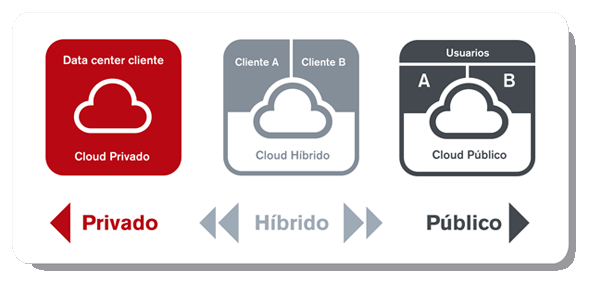
\includegraphics[width=0.7\textwidth]{Imagenes/Bitmap/cloud0}
    \caption{Modelos de despliegue de la computación en la nube}
    \label{fig:cloud1}
\end{figure}

\subsubsection{Tipos de nubes por el modelo de servicio}
Según \cite{nist} se ofrecen tres modelos de servicio:
\begin{enumerate}
    \item \textbf{Software as a Service - SaaS}.- Al usuario se le ofrece la
          capacidad de que las aplicaciones  que  su  proveedor  le  suministra
          corran  en  una  infraestructura cloud, siendo las aplicaciones accesibles
          a través de, por ejemplo, un navegador web como en el caso del webmail,
          que es posiblemente el ejemplo más representativo, por lo extendido,
          de este modelo de servicio. El usuario carece de cualquier control sobre
          la infraestructura o sobre las propias aplicaciones, excepción hecha
          de las posibles configuraciones de usuario o personalizaciones que se
          le permitan.
    \item \textbf{Platform as a Service}.- Al usuario se le permite desplegar
          aplicaciones propias  (ya  sean  adquiridas  o  desarrolladas  por  el
          propio  usuario)  en  la  infraestructura cloud de  su  proveedor, que
          es  quien  ofrece  la  plataforma  de desarrollo y las herramientas de
          programación. En este caso, es el usuario quien mantiene el control de
          la aplicación, aunque no de toda la infraestructura subyacente.
    \item \textbf{Infrastructure as a Service}.- El proveedor ofrece al usuario
          recursos como capacidad  de  procesamiento,  de  almacenamiento,  o
          comunicaciones, que el usuario puede utilizar para ejecutar cualquier
          tipo de software, desde sistemas operativos hasta aplicaciones.
\end{enumerate}

\begin{figure}[h]
    \centering
    \captionsetup{justification=centering}
    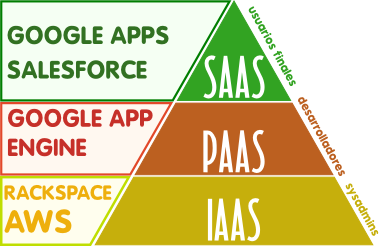
\includegraphics[width=0.7\textwidth]{Imagenes/Bitmap/cloud1}
    \caption{Modelos de servicio de la computación en la nube con algunos proveedores en cada tipo.}
    \label{fig:cloud1}
\end{figure}

Por otro lado \cite{msolutions} define estos 3 tipos de nubes por el modelo de servicio
de la siguiente forma:
\begin{enumerate}
    \item \textbf{IaaS}: Modelo de servicios en el que al cliente se le ofrece tanto un
          medio de almacenamiento básico como una serie de capacidades de cóputo en la red.
          Todo ello haciendo uso de sistemas operativos virtualizados y servidores ubicados
          en la nube a los que el usuario accede a través de la red.
    \item \textbf{PaaS}: Modelo de servicios en el que al cliente se le ofrece un entorno
          dedicado exclusivamente al desarrollo de aplicaciones. El proveedor de dicho servicio será
          el encargado de proporcionar la red, los servidores y el almacenamiento necesario.
    \item \textbf{SaaS}: Modelo de servicios en el que al cliente se le proporcionan ciertas aplicaciones
          a través de Internet. Tanto el \emph{software} como los datos empleados por el usuario
          quedan alojados en los servidores del proveedor de servicios en la nube, accediendo el cliente
          a ellos mediante un navegador web.
\end{enumerate}
\subsubsection{Beneficios de la computación en la nube}
Respecto a los beneficios de la computación en la nube \cite{cierco} indica que los beneficios
del cloud son muy relevantes desde distintos puntos de vista.
Para la economía global, el traslado de las economías de escala de los
proveedores a las empresas usuarias reduce los costes globales en TI, elimina
las barreras de entrada para nuevos actores y dinamiza la economía, promoviendo
la aparición de nuevos modelos de negocio y lineas de actividad, facilitando
por la creación de empresas y de empleo.
%%-------- Servicios web
\subsubsection{Servicios web}

Según \cite{w3c} define a los servicios web como un sistema de software diseñado
para soportar interacción interoperable máquina a máquina a traves de una red.
Por su parte
%%-------- aplicaciones moviles
%%-------- smarth phone
%%-------- Internet
\subsubsection{Internet}
Según \cite{fnc} Internet hace referencia a un sistema global de información que:
\begin{enumerate}[i.]
    \item Esta relacionado lógicamente por un único espacio de direcciones
          global basado en el protocolo de Internet(IP) o en sus extensiones
    \item Es capaz de soportar comunicaciones usando el conjunto de protocolos TCP/IP
          o sus extensiones u otros protocolos compatibles con IP, y
    \item Emplea, provee o hace accesible, privada o públicamente, servicios de
          alto nivel en capas de comunicaciones y otras infraestructuras relacionadas
          aqui descritas.
\end{enumerate}
%%-------- Intranet
\subsubsection{Intranet}
Según \cite{lafrance} una Intranet no es más que una Internet privada, interior a una
organización y protegida de las miradas indiscretas por una barrera (firewall) que
impide a cualquier intruso conocer su red informática interna.
%%-------- virtualizacion
%%-------- Digitalizacion
%%-------- Ovicuidad
%%-------- API
%%-------- modelos de negocio en la nube
%%-------- seguridad en la nube
%%-------- tercerizacion u outsourcing
%%-------- riesgos y amenazas
%%-------- SLA
\subsubsection{Acuerdo de nivel de servicio}
Según \cite{qianq}, un acuerdo de nivel de servicio es usado por las partes
involucradas en un negocio electronico donde los requerimientos minimos y obligaciones son
plasmados en él incluyendo los socios de negocio, politica de precios y las propiedad
de los recursos necesarios para la prestacion del servicio de negocio.

Además \cite{qianq} agrega que los precios parecen ser la caracteristica dominante
de un acuerdo de nivel de servicio, otros asuntos como la disponiblidad, seguridad,
calidad del servicio se convierten en cruciales en este tipo de contratos.

Cabe aclarar que nos podemos referir a estos acuerdos con la abreviatura ANS o SLA,
este ultimo de su traduccion inglesa (Service Layer Agreement).
%%-------- redes sociales

%%-------- Multitenencia
\subsubsection{Multitenencia}

Según \cite{chandra} la multitenencia es una caracteristicas esencial de los
sistemas en la nube que apunta a proveer aislamiento de diferentes usuarios de
ese sistema en la nube (inquilinos) mientras se maximiza el uso de recursos compartidos.
Además \citep{chandra} que se espera que esa multitenencia sea soportada en varios niveles de la infraestructura
de la nube, por ejemplo en el nivel de aplicación, la multitenencia es la que permite
que una sola instancia de una aplicación pueda escalar para satisfacer a muchos
usuarios al mismo tiempo.

La definción anterior quiere decir que se busca el maximo uso de los recursos
disponibles mientras que los usuarios tengan la sensacion de que usan recursos
independientes.
%%-------- privacidad de los datos
%%-------- seguridad
%%-------- licencia de software
\subsubsection{Licencia de software}
Según \cite{moro} una licencia de software es un contrato entre el autor o el titular
de los derechos de explotación de un programa informático y el usuario (un particular
o una empresa), un contrato que regula los términos en los que este último puede
utilizar el software cumpliento los términos y las clausulas de la licencia.

Al respecto debemos mencionar que todos las aplicaciones de software tienen una
licencia, algunas de estas licencias son más permisivas que otras. Algunas de estas
son totalmente abiertas (es decir que permiten hacer cualquier cosa con el aplicativo).
%%-------- interoperatividad
\subsubsection{Interoperabilidad}
Según \cite{kajan} la interoperabilidad es la habilidad de dos o más sistemas o
componentes para intercambiar información y usar esa información que fue intercambiada.
%%-------- aplicaciones
\subsubsection{Aplicaciones de software}

Según \cite{pablos} las aplicaciones son programas diseñados para ejecutar
trabajos o procesos de cálculo específico que precisa el usuario o a la unidad
empresarial.
%%-------- migracion a la nube
%%-------- frontend
%%-------- backend
%%-------- internet de las cosas
%%-------- brecha digital
%%-------- aplicaciones web
\subsubsection{Aplicaciones web}
Según \cite{nino} las aplicaciones web son aplicaciones a las que accede mediante un
navegador y están alojadas en servidores dentro de una Intranet o en Internet.

Además \cite{nino} agrega que las principales ventajas de las aplicaciones web de
escritorio son:
\begin{itemize}
    \item Se pueden ejecutar desde cualquier equipo informático siempre que tenga
          una conexión a Internet o a la Intranet.
    \item No es necesario utilizar un sistema operativo en concreto, cualquiera sirve.
    \item No hay que instalar ningún programa, con el navegador es suficiente.
    \item No hay que preocuparse del espacio ocupado por los datos, de eso se encarga
          el servidor.
    \item La información puede ser compartida simultáneamente por .
    \item Se realizan copias de seguridad de la información almacenada en el servidor.
    \item Las aplicaciones suelen estar actualizadas en los servidores, algunas
          aplicaciones avisan cuando una actualización disponible.
    \item
\end{itemize}

%% ------------------------------- GESTION EMPRESARIAL ------------------------
\subsection{Gestión Empresarial}
\subsubsection{Administración de empresas}
Según \cite{koontz} la administración es el proceso mediante el cual se diseña
y mantiene un ambiente en el que individuos que trabajan en grupos cumplen metas
especificas de manera eficaz. Por otra parte \citep{galindo} define la administración
como el proceso cuyo objeto es la coordinación eficaz y eficiente de los recursos
de un grupo social para lograr sus objetivos con la máxima productividad.
En ambas deficiones se hace hincapié en los terminos eficacia y logro de objetivos
ya que ambos persiguen obtener los mejores resultados posibles con la cantidad
minima de recursos tanto materiales como humanos. Por su parte \citep{chiavenato}
señala que la tarea de la administración consiste en interpretar los objetivos
de la empresa y transformarlos en acción empresarial mediante planeación, organización,
dirección y control de las actividades realizadas en las diversas áreas y niveles
de la empresa para conseguir tales objetivos. Por tanto, administración es el
proceso de planear, organizar, dirigir y controlar el empleo de los recursos
organizacionales para conseguir determinados objetivos con eficiencia y eficacia.

\subsubsection{Proceso administrativo}
\cite{chiavenato} cita a \citep{fayol} quien define el acto de administrar como
\emph{planear, organizar, dirigir, coordinar y controlar}. Las funciones administrativas
abarcan los elementos de la administración, es decir, las funciones del administrador
(véase la imágen \ref{fig:adm}):
\begin{enumerate}
    \item \emph{Planeación}: avisorar el futuro y trazar el programa de acción.
    \item \emph{Organización}: construir las estructuras materiales y sociales de
          la empresa.
    \item \emph{Dirección}: guiar y orientar al personal.
    \item \emph{Coordinación}: enlazar, unir y armonizar todos los actos y esfuerzos
          colectivos.
    \item \emph{Control}: verificar que todo suceda de acuerdo con las reglas establecidas
          y las órdenes dadas.
\end{enumerate}

\subsubsection{Funciones de la empresa}
\cite{chiavenato} cita a \cite{fayol}, indicando que toda empresa cumple seis funciones
(véase la imágen \ref{fig:adm}):
\begin{enumerate}
    \item \emph{Funciones técnicas}, relacionadas con la producción de bienes o
          servicios de la empresa.
    \item \emph{Funciones comerciales}, relacionadas con la compra, la venta o el
          intercambio.
    \item \emph{Funciones financieras}, relacionadas con la búsqueda y gestión
          de capitales.
    \item \emph{Funciones de seguridad}, relacionadas con la protección y preservación
          de los bienes y las personas.
    \item \emph{Funciones contables}, relacionadas con los inventarios, los registros,
          los balances, los costos y las estadísticas.
    \item \emph{Funciones administrativas}, relacionadas con la integración de las
          otras cinco funciones en la dirección. Las funciones administrativas
          coordinan y sincronizan las demás funciones de la empresa, y están siempre
          por encima de ellas.
\end{enumerate}

\begin{figure}[h]
    \centering
    \captionsetup{justification=centering}
    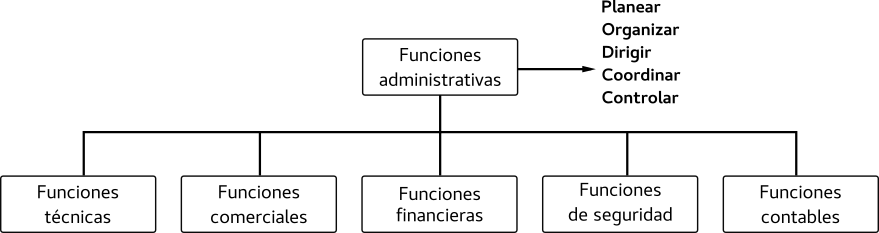
\includegraphics[width=1.0\textwidth]{Imagenes/Bitmap/funciones_adm}
    \caption{Proceso administrativo y funciones de la administración según Fayol}
    \label{fig:adm}
\end{figure}

\subsubsection{Gestión}
Según \cite{beltran} define el termino gestión como el conjunto de decisiones
y acciones que llevan al logro de objetivos previamente establecidos.

Además \cite{beltran} considera la gestión en tres niveles diferentes:
\begin{enumerate}
    \item \textbf{Gestión estratégica}: Se desarrolla en la dirección, y tiene como
          característic fundamental que la influencia de las acciones y las decisiones
          es, generalmente, corporativa y de largo plazo.
    \item \textbf{Gestión táctica}: Se desarrolla con base en la gestión
          estratégica. El impacto de las decisiones y acciones, de mediano plazo,
          abarca las unidades estratégicas del negocio.
    \item \textbf{Gestión operativa}: Se desarrolla con base en la gestión
          táctica. El impacto de la decisiones y acciones es de corto plazo e incluye
          los equipos naturales de trabajo y los individuos. Básicamente tiene
          que ver con la funciones de ejecución y control.
\end{enumerate}

\subsubsection{Control de gestión}
% TODO : Citar a la fuente original
Según \cite{beltran} el control de gestión es un instrumento gerencial, integral
y estratégico que, apoyado en indicadores, índices y cuadros producidos en forma
sistemática, periódica y objetiva, permite que la organización sea efectiva para
captar recursos, eficiente para transformarlos y eficaz para canalizarlos.

Por otro lado, \cite{beltran} agrega que un sistema de control de gestión tiene
como objetivo facilitar a los administradores con responsabildades de planeación
y control de cada grupo operativo, información permanente e integral sobre su desempeño,
que les permita a éstos autoevaluar su gestión y tomar los correctivos del caso.



\subsubsection{Gestión de inventarios}
Según \cite{rae} un inventario es un asiento de los bienes y demás cosas
pertenecientes a una persona o comunidad, hecho con orden y precisión.

Según \cite{meza} el inventario de mercaderías se compone de los bienes de la
empresa compra para luego venderlos. Esta de definición se aplica a empresas
comerciales (empresas que comprar un producto para luego venderlo).

Además de la definición anterior \cite{meza} indica que las empresas manufactureras
(fábricas) tienen tres inventarios: materia prima, productos en proceso y productos
terminados.

Sin embargo \cite{chapman} indica, según su propio criterio, que la segunda categoria de la división se basa
en la \emph{posición del inventario en el proceso}, la primera se basa en la
\emph{fuente de la demanda}. Bajo este segundo criterio existen cuatro subcategorias
generales:
\begin{itemize}
  \item La \textbf{materia prima} constituye el inventario que debe adquirirse para
        utilizarlo en el proceso de producción, y que no tiene un valor añadido
        por el proceso de producción de la compañia.
  \item El \textbf{trabajo en proceso (TEP)} representa el inventario que ya ha recibido
        algún valor agregado, pero que todavía debe sufrir un procesamiento
        adicional antes de poder utilizarlo para atender la demanda de los clientes.
  \item Los \textbf{bienes terminados} representan el inventario de aquellos productos
        que han pasado ya por todo el procesamiento de parte de la empresa. Por lo general
        dicho inventario se encuentra listo(con la posible excepción del empaque)
        para atender con él la demanda de los clientes.
  \item El inventario de \textbf{mantenimiento, reparación y operaciones (MRO)}
        es el acervo de material que se utiliza para dar apoyo a los procesos productivos
        y de negocio de la empresa, pero por lo general no esta destinado a la venta
        directa al público. Se compone de partes de repuesto, aceite para maquinaria,
        suministros de limpieza, suministros de oficina, etc.
\end{itemize}

Las definiciones de \cite{meza} y \citep{chapman} son similares, salvo el tipo de
almacen extra en el segundo caso, pero ambas señalan de manera muy aproximada los
tipos de inventarios, o almacenes, que podemos observar en las empresas de la ciudad
del Cusco.

\subsubsection{Indicadores de gestión}
Previamente \cite{beltran} define indicador coo la relación entre las variables
cuantitativas o cualitativas que permiten observar la situación y las tendencias
de cambio generadas en el objeto o fenómeno observado, respecto de los objetivos
y metas previstos e influencias esperadas.

Respecto a esto \cite{silva} agrega que uno de los objetivos principales de los
indicadores de gestión consiste en establecer un sistema de instrumentos que
permita en forma rápida y proactiva, administrar la empresa y hacer posible la
comparación de los resultados con la metas propuestas y de igual forma definir
parámetros que permitan que el diseño de los objetivos, los planes y las metas sean
reales en el tiempo para controlar las operaciones diarias que se realizan dentro
de la empresa. También crear mecanismos de detección de fallas que garanticen
la posibilidad de llevar a cabo acciones concretas que permitan obtener soluciones
reales y de aplicación inmediata.

Según \cite{beltran}, los indicadores de gestión son, ante todo, información, es
decir, agregan valor, no son solo datos. Siendo información, los indicadores de
gestión deben tener los atributos de la información, tanto en forma individual
como cuando se presentan agrupados.

En los parrafos anteriores queda de manifiesto la importancia de los indicadores
de gestión como instrumentos que permiten determinar la situación actual de la
empresa en distintos aspectos y a la vez permiten fijar las estrategias futuras
para que estas sean alcanzables en el tiempo.

\subsubsection{Características de los indicadores}
Según \cite{silva} los indicadores de gestión deben cumplir con unos requisitos
y elementos para poder apoyar la gestión para conseguir el objetivo, las cuales
pueden ser:
\begin{enumerate}
    \item \emph{Simplicidad}, se puede entender como la capacidad para definir el
          evento que se pretende medir de manera poco costosa en tiempo y recurso.
    \item \emph{Validez en el tiempo}, Puede definirse como la propiedad de ser
          permanente en un periodo deseado.
    \item \emph{Adecuación}, Corresponde a la facilidad de la medida para describir
          por completo el fenómeno o efecto. Debe reflejar la magnitud del hecho
          analizado y mostrar la desviación real del nivel deseado.
    \item \emph{Utilidad}, es la posibilidad del indicador para estar siempre
          orientado a buscar las causas que han llevado a que alcance un valor
          particular y mejorarlas.
    \item \emph{Participación de los usuarios}, es la habilidad para estar involucrados
          desde el diseño, y debe proporcionarseles los recursos y formación necesarios
          para su ejecución.
    \item \emph{Oportunidad}, es la capacidad para que los datos sean recolectados
          a tiempo, igualmente se requiere que la información sea analizada oportunamente
          para poder actual.
\end{enumerate}

\subsubsection{Indicadores del negocio con base en el esquema de valor de negocio}
Según \cite{cruz} para la identificación de variables e indicadores del negocio
se considera inicialmente el ESQUEMA DE VALOR DE MERCADO, los cuales están asociados
generalmente con la misión y sus elementos cuantificables como de las estrategias,
y luego son transformados en indicadores básicos, clave y operativos.

Además \cite{cruz} agrega que el esquema de valor de mercado de una empresa está
soportado por cuatro (4) grandes macroindicadores: rentabilidad, competitividad,
riesgo y liquidez. Todos ellos, excepto el riesgo, son de signo creciente, es
decir mejoran al crecer de valor.

\begin{figure}[t]
    \begin{center}
        \includegraphics[width=1.0\textwidth]%
        {Imagenes/Vectorial/valor}
        \caption{Esquema de valor de mercado}
        \label{fig:indicadores_valor_mercado}
    \end{center}
\end{figure}

\subsubsection{Indicador de Efectividad}
Según \cite{cruz} la efectividad, significa cuantificación del logro de la meta,
también es sinónimo de eficacia y se le define como \emph{Capacidad de lograr el
efecto que se desea}. Los indicadores de eficacia o efectividad, tienen que ver
con hacer realidad un intento o propósito, y están relacionados con el cumplimiento
al ciento por ciento de los objetivos planteados.

\cite{cruz} ubica a la efectividad respecto a los indicadores del negocio con base
en el esquema de valor de mercado de la figura \ref{fig:indicadores_valor_mercado}
como parte de la Rentabilidad, tal como se puede ver en la figura \ref{fig:efectividad}

Además \cite{cruz} señala que se pueden diseñar indicadores de efectividad
como el de las formulas \ref{eq:calc_efectividad_instalaciones} y \ref{eq:calc_efectividad_ventas}
pero éstos no son únicos.

\begin{figure}[t]
    \begin{center}
        \includegraphics[width=0.8\textwidth]%
        {Imagenes/Vectorial/efectividad}
        \caption{Efectividad}
        \label{fig:efectividad}
    \end{center}
\end{figure}

\begin{equation}\label{eq:calc_efectividad_instalaciones}
\text{Efectividad en las instalaciones} = \frac{\text{Vol}_{\text{producido}}}{\text{Vol}_{\text{programado}}} \times{100}
\end{equation}

\begin{equation}\label{eq:calc_efectividad_ventas}
\text{Efectividad en ventas} = \frac{\text{Vol}_{\text{vendido}}}{\text{Vol}_{\text{planificado}}} \times{100}
\end{equation}

\cite{cruz} agrega la especificación de los indicadores de efectividad mostradolos
en la tabla \ref{t:efectividad}.

\begin{table}
    \begin{tabular}{|p{8cm}|p{5cm}|}
        \hline
        \thead{Descripción del Indicador} & \thead{Variables fundamentales} \\ \hline
        \begin{minipage}{3in}
            \textbf{Efectividad en el uso de instalaciones}\\
            Es el grado de cumplimiento del programa de
            producción. Este factor puede estar afectado por
            causas imputadas tanto a los equipos de producción, como a los que administran el proceso. El
            indicador es medido porcentualmente ( \%).
        \end{minipage}
         &
        \begin{minipage}{2in}
            \vskip 4pt
            \begin{enumerate}
                \item Disponibilidad de las instalaciones.
                \item Eficiencia de los equipos.
                \item Efectividad en la logistica y transporte.
            \end{enumerate}
            \vskip 4pt
        \end{minipage}
        \\
        \hline
        \begin{minipage}{3in}
            \textbf{Efectividad en las ventas}\\
            Es el grado de cumplimiento del plan de ventas, en términos de
            volumen despachado, tanto para el mercado nacional como para
            exportación, así como el total. El indicador es medido
            porcentualmente (\%).
        \end{minipage}
         &
        \begin{minipage}{2in}
            \vskip 4pt
            \begin{enumerate}
                \item Efectividad en el uso de las instalaciones.
                \item Eficiencia en la gesión de comercialización y ventas.
            \end{enumerate}
            \vskip 4pt
        \end{minipage}
        \\
        \hline
    \end{tabular}
    \caption{Especificación de los indicadores de efectividad}
    \label{t:efectividad}
\end{table}

\subsubsection{Indicador de eficiencia}
Según \cite{cruz} la eficiencia es la capacidad administrativa de producir el
máximo de resultados con el mínimo de recursos, el mínimo de energía y en el
mínimo de tiempo posible.

\cite{cruz}, tambien muestra la relacion de la eficiencia y la rentabilidad de la
figura \ref{fig:indicadores_valor_mercado} por medio de la figura \ref{fig:eficiencia}.

Además \cite{cruz} indica que entre los indicadores de eficiencia se pueden
mencionar los de las ecuaciones \ref{eq:calc_eficiencia_capacidad_instalada}, \ref{eq:calc_eficiencia_capacidad_instalada}

\begin{figure}[t]
    \begin{center}
        \includegraphics[width=0.7\textwidth]%
        {Imagenes/Vectorial/eficiencia}
        \caption{Eficiencia}
        \label{fig:eficiencia}
    \end{center}
\end{figure}

\begin{equation}\label{eq:calc_eficiencia_capacidad_instalada}
    \text{Uso de la capacidad instalada}=\frac{\text{Volumen de producción}}{\text{Capacidad instalada}} \times{100}
\end{equation}

\begin{equation}\label{eq:calc_eficiencia_capacidad_instalada}
    \text{Nivel de inventarios}=\frac{\text{Costo del inventario}}{\text{Ventas netas}} \times{100}
\end{equation}

Además \cite{cruz} muestra la especificación del indicador mencionando su
descripción y sus variables en la tabla \ref{t:eficiencia}.

\begin{table}
    \begin{tabular}{|p{5cm}|p{8cm}|}
        \hline
        \thead{Descripción del Indicador} & \thead{Variables fundamentales} \\ \hline
        \begin{minipage}{2in}
            \textbf{Uso de la capacidad instalada}\\
            Indica el uso racional de las instalaciones productivas, con base en
            la capacidad nominal o instalada. El indicador es medido porcentualmente (\%).
        \end{minipage}
         &
        \begin{minipage}{3in}
            \vskip 4pt
            \begin{enumerate}
                \item Disponibilidad de las instalaciones.
                \item Eficiencia en el mantenimiento.
                \item Efectividad en el transporte.
                \item Capacidad de las instalaciones.
            \end{enumerate}
            \vskip 4pt
        \end{minipage}
        \\
        \hline
        \begin{minipage}{2in}
            \textbf{Nivel de inventarios}\\
            Permite conocer el uso racional del capital invertido en inventarios
            con relación a las ventas netas. El indicador es medido porcentualmente (\%).
        \end{minipage}
         &
        \begin{minipage}{3in}
            \vskip 4pt
            \begin{enumerate}
                \item Eficiencia en el uso de los insumos.
                \item Determinación optima de los niveles de reposición.
                \item Efectividad en el pago a proveedores.
                \item Eficiencia en el tiempo de compras.
            \end{enumerate}
            \vskip 4pt
        \end{minipage}
        \\
        \hline
    \end{tabular}
    \caption{Especificación de los indicadores de eficiencia}
    \label{t:eficiencia}
\end{table}

\subsubsection{Indicador de calidad}
Según \cite{cruz} el concepto técnico de calidad representa más bien una forma
de hacer las cosas en las que, fundamentalmente, predominan la preocupación por
satisfacer al cliente y por mejorar, día a día, procesos y resultados. Hoy en día
introduce el concepto de mejora continua en cualquier organización y a todos los
niveles de la misma. Entre los indicadores de eficiencia se pueden mencionarlos
siguientes:

\begin{figure}[t]
    \begin{center}
        \includegraphics[width=0.7\textwidth]%
        {Imagenes/Vectorial/calidad}
        \caption{Calidad}
    \end{center}
\end{figure}

\begin{equation}\label{eq:rendimiento_calidad}
    \text{Rendimiento de calidad}=\frac{\text{Vol}_{\text{producción conforme}}}{\text{Vol}_{\text{total producido}}} \times{100}
\end{equation}

\begin{equation}\label{eq:calidad_uso}
    \text{Calidad de uso}=\frac{\text{Volumen reclamado por calidad (procedente)}}{\text{Volumen total de ventas}} \times{100}
\end{equation}

\begin{table}
    \begin{tabular}{|p{5cm}|p{8cm}|}
        \hline
        \thead{Descripción del Indicador} & \thead{Variables fundamentales} \\ \hline
        \begin{minipage}{2in}
            \textbf{Relación deuda/calidad}\\
            Mide el nivel de apalancamiento del negocio, con recursos externos
            con base en el patrimonio. El indicador es medido porcentualmente (\%).
        \end{minipage}
         &
        \begin{minipage}{3in}
            \vskip 4pt
            \begin{enumerate}
                \item Efectividad en el uso de las instalaciones.
                \item Tiempo efectivo de trabajo.
                \item Cumplimiento plan de desarrollo y capacitación.
                \item Eficiencia en la gestión de calidad.
            \end{enumerate}
            \vskip 4pt
        \end{minipage}
        \\
        \hline
    \end{tabular}
    \caption{Especificación de los indicadores de calidad}
    \label{t:calidad}
\end{table}

\subsubsection{Indicador de productividad}
Según \cite{cruz} los indicadores de productividad son los siguientes:

\begin{figure}[t]
    \begin{center}
        \includegraphics[width=1.0\textwidth]%
        {Imagenes/Vectorial/productividad}
        \caption{Productividad}
    \end{center}
\end{figure}

\begin{equation}\label{eq:productividad_mano_obra}
    \text{Productividad de mano de obra}=\frac{\text{Vol}_{\text{producción conforme}}}{\text{Horas hombre trabajadas}}
\end{equation}

\begin{equation}\label{eq:productividad_costo_unitario}
    \text{Costo Unitario de Producción} = \frac{\text{Costo total de producción}}{\text{Volumen de producción conforme}}
\end{equation}

\begin{equation}\label{eq:productividad_capital}
    \text{Productividad del capital} = \frac{\text{Volumen de producción conforme}}{\text{Activo total promedio}}
\end{equation}

\begin{table}
    \begin{tabular}{|p{7cm}|p{7cm}|}
        \hline
        \thead{Descripción del Indicador} & \thead{Variables fundamentales} \\ \hline
        \begin{minipage}{2.5in}
            \textbf{Rentabilidad total}\\
            Es la rentabilidad medida en términos de la capacidad de generar
            utilidades con los activos disponibles. El indicador es medido
            porcentualmente (\%). \\
            \textbf{Margen neto}\\
            Mide la rentabilidad en función de las ventas generadas. El
            indicador es medido porcentualmente (\%). \\
            \textbf{Rotación del activo} \\
            Mide las veces que en un año se mueve el activo de la empresa y
            muestra la intensidad con que los activos totales se están utilizando.\\
            \textbf{Margen de operaciones} \\
            Mide las ganancias en operaciones en función de las ventas generadas,
            sin tomar en cuenta la carga financiera y los impuestos. El indicador
            es medido porcentualmente (\%).
        \end{minipage}
         &
        \begin{minipage}{2.5in}
            \vskip 4pt
            \begin{enumerate}
                \item Cumplimiento del Plan de Ventas.
                \item Efectividad en el Plan de Producción.
                \item Cumplimiento en la ejecución presupuestaria.
                \item Eficiencia en el uso de los recursos.
                \item Eficiencia en la gestión de comercialización y ventas.
                \item Control efectivo de los activos y pasivos.
                \item Administración de los programas de reducción de costos.
                \item Eficiencia en la gestión de calidad.
            \end{enumerate}
            \vskip 4pt
        \end{minipage}
        \\
        \hline
    \end{tabular}
    \caption{Especificación de los indicadores de rentabilidad}
    \label{t:rentabilidad}
\end{table}

\subsubsection{Indicador de apalancamiento}
Según \cite{cruz} los indicadores de apalancamiento son los siguientes:

\begin{figure}[t]
    \begin{center}
        \includegraphics[width=1.0\textwidth]%
        {Imagenes/Vectorial/apalancamiento}
        \caption{Apalancamiento}
    \end{center}
\end{figure}

\begin{equation}\label{apalancamiento}
    \text{Relación deuda/capital} = \frac{\text{Deuda total}}{\text{Patrimonio}}\times{100}
\end{equation}

\subsubsection{Indicadores de rentabilidad}
Según \cite{cruz} los indicadores de rentabilidad son:

\begin{figure}[t]
    \begin{center}
        \includegraphics[width=1.0\textwidth]%
        {Imagenes/Bitmap/rentabilidad01}
        \caption{Rentabilidad}
    \end{center}
\end{figure}

\begin{equation}\label{eq:rentabilidad_total}
    \text{Rentabilidad total}=\frac{\text{Utilidad total}}{\text{Activo total promedio}}\times{100}
\end{equation}

\begin{equation}\label{eq:margen_neto}
    \text{Margen neto}=\frac{\text{Utilidad neta}}{\text{Ventas netas}}\times{100}
\end{equation}

\begin{equation}\label{eq:rotacion_activo}
    \text{Rotación del activo (veces)}=\frac{\text{Ventas netas}}{\text{Activo total promedio}}
\end{equation}

\begin{equation}\label{eq:margen_operaciones}
    \text{Margen operaciones} = \frac{\text{Utilidad en operaciones}}{\text{Ventas netas}}\times{100}
\end{equation}

\begin{table}
    \begin{tabular}{|p{5cm}|p{7.5cm}|}
        \hline
        \thead{Descripción del Indicador} & \thead{Variables fundamentales} \\ \hline
        \begin{minipage}{2in}
            \textbf{Riesgo operativo}\\
            Posibilidad de no estar en capacidad de cubrir los costos de operación.
            También mide el peligro de no ganar. \\
            \textbf{Riesgo financiero}\\
            Posibilidad de no estar en condiciones de cubrir los costos de financieros,
            o sea mide el peligro a que está expuesta la empresa de no pagar sus deudas. \\
        \end{minipage}
         &
        \begin{minipage}{3in}
            \vskip 4pt
            \begin{enumerate}
                \item Cumplimiento del Plan de Ventas.
                \item Efectividad en el Plan de Producción.
                \item Cumplimiento en la ejecución presupuestaria.
                \item Eficiencia en el uso de los recursos.
                \item Eficiencia en la gestión de comercialización y ventas.
                \item Administración de los programas de reducción de costos.
                \item Eficiencia en la gestión de calidad.
            \end{enumerate}
            \vskip 4pt
        \end{minipage}
        \\
        \hline
    \end{tabular}
    \caption{Especificación de los indicadores de riesgo}
    \label{t:riesgo}
\end{table}

\subsubsection{Indicadores de riesgo}
\cite{cruz} indica que si la empresa no cotiza en la bolsa y sus acciones no tienen
variabilidad estadística, por supuesto, no se tienen los soportes para calcular
los indicadores de riesgo, pero no implica que no tengan riesgos, por lo tanto
es posible establecer un indicador de riesgo empresarial, entendiendo por este
la posibilidad de que la organización no pueda cubrir sus costos de operación
y/o financieros.

En este sentido \cite{cruz} señala que el indicador tiene su base en las
utilidades antes de intereses e impuestos que pueda tener la empresa, a fin de
cubrir sus costos de operación (fijos y variables) y las utilidades antes de
impuestos, a fin de cubrir sus costos financieros.

En este sentido \cite{cruz} distingue dos tipos de riesgos:
\begin{itemize}
    \item \emph{RIESGO OPERATIVO}, posibilidad de no estar en capacidad de cubrir
          los costos de operación. También mide el peligro de no ganar en las
          operaciones.
    \item \emph{RIESGO FINANCIERO}, posibilidad de no estar en condiciones de
          cubrir los costos de financieros, o sea mide el peligro a que está
          expuesta la empresa de no pagar sus deudas.
\end{itemize}

Dado esto \cite{cruz} establece indicadores de riesgo operativo y financiero en las
formulas \ref{eq:riesgo1} y \ref{eq:riesgo2}.

\begin{equation}\label{eq:riesgo1}
    \text{Riesgo operativo} = \text{Utilidad en operaciones} \geq 0
\end{equation}

\begin{equation}\label{eq:riesgo2}
    \text{Riesgo financiero} = \text{Utilidad antes de impuestos} \geq 0
\end{equation}

\subsubsection{Indicadores de competitividad}
Según \cite{cruz} se entiende por competitividad a la capacidad de una organización
pública o privada, lucrativa o no, de mantener sistemáticamente ventajas comparativas
que le permitan alcanzar, sostener y mejorar una determinada posición en el entorno
socioeconómico.

\cite{cruz} define los indicadores en las formulas \ref{eq:competitividad1} y
\ref{eq:competitividad2}.

\begin{equation}\label{eq:competitividad1}
    \text{Comp. CU del producto} = \frac{\text{Costo producto propio}}{\text{Costo producto competidor}} \times{100}
\end{equation}

\begin{equation}\label{eq:competitividad2}
    \text{Var. participación en mercado} = \frac{\text{Participación año anterior}}{\text{Participación año actual}}\text{100}
\end{equation}

%\subsubsection{Liquidez}
%\subsubsection{mipyme}
%\subsubsection{emprendimiento}
\newpage
\section{Hipótesis}

\subsection{Hipótesis General}

Existe un efecto positivo del uso de la computación en la nube en la
gestión de las micro, pequeñas y medianas empresas pertenecientes al Centro de
Desarrollo Empresarial del Cusco.

\subsection{Hipótesis Espec'ificas}
\begin{enumerate}[a., noitemsep]
    % preguntaar si es necesario colocar las palabras pe-post implementacion
    \item El nivel de gestión de las MiPYMES pertenecientes al Centro de Desarrollo
          Empresarial del Cusco antes del uso de las herramientas de la computación
          en la nube es deficiente.
    \item El nivel de gestión de las MiPYMES pertenecientes al Centro de Desarrollo
          Empresarial del Cusco después del uso de las herramientas de la computación
          en la nube es eficiente.
    \item El efecto del uso de herramientas de la computación en la nube en la
          gestión de las MiPYMES pertenecientes al Centro de Desarrollo Empresarial
          del Cusco es positiva.
\end{enumerate}

\section{Variables}

\subsection{Identificación de variables}
Según \cite{sampieri} una variable es una propiedad que puede fluctuar y cuya
variación es suceptible de medirse u observarse. Además agrega que las variables
adquieren valor para la investigación cientifica cuando llegan a relacionarse
con otras variables.

Respecto al tipo de investigación preexperimental \cite{sampieri} indica que deben
su nombre a que el grado de control es mínimo y que además consiste en administrar
un estímulo o tratamiento a un grupo, en este caso \emph{el uso de las herramientas
de la computación en la nube}, y después aplicar una medición de una o más
variables, en este caso \emph{la gestión empresarial}, para observar cuál es
el nivel del grupo  en éstas. En ese entender, la unica variable identificada es
\emph{\textbf{Gestión Empresarial.}}
%-----------------
\subsection{Operacionalización de variables}
Tal como se menciono en la sección anterior, la única variable encontrada es
\emph{\textbf{gestión empresarial}}, cuyo análisis se muestra en la tabla \ref{t:gestion}.
\begin{sidewaystable}[htbp]
    \centering
    \caption{Operacionalización de la variable ``\emph{Gestión empresarial}''}
    \label{t:gestion}
    \begin{tabular}{|p{3cm}|p{4cm}|p{3.5cm}|p{3.5cm}|p{5cm}|}
    \hline
    \thead{Variable} & \thead{Definición\\Conceptual} & \thead{Definición\\Operacional} & \thead{Dimensiones} & \thead{Indicadores} \\ \hline
    \multirow{1}{3cm}{Gestión empresarial} &
    \multirow{5}{4cm}{La administración es el proceso mediante el cual se diseña
            y mantiene,un ambiente, en el que individuos que trabajan en grupos,
            cumplen metas,especificas de manera eficaz\citep{koontz}} &
    \multirow{5}{3.5cm}{Según \cite{fayol} toda empresa posee seis funciones básicas:
    \begin{itemize}[noitemsep]
      \item Funciones técnicas.
      \item Funciones comerciales.
      \item Funciones financieras.
      \item Funciones de seguridad.
      \item Funciones contables.
      \item Funciones administrativas.
    \end{itemize}
    }
     &
    Producción (funciones de seguridad y técnicas) &
    \begin{itemize}[noitemsep]
      \item Inventario.
      \item Volumen de producción.
      \item Procesos.
    \end{itemize} \\ \cline{4-5}
     &  &  & Comercialización (función comercial) &
     \begin{itemize}[noitemsep]
       \item Clientes.
       \item Proveedores.
     \end{itemize} \\ \cline{4-5}
     &  &  & Administración (funciones contables y financieras) &
     \begin{itemize}[noitemsep]
       \item Herramientas de gestión.
       \item Control de ingresos y egresos.
       \item Estados financieros.
       \item Ratios.
       \item Liquidez.
     \end{itemize} \\ \hline
    \end{tabular}
    * Dimensiones adaptadas de acuerdo a las funciones de la empresa según \cite{fayol}.
\end{sidewaystable}

\newpage
\section{Definici\'on de t\'erminos b\'asicos}
\begin{itemize}
  \item \textbf{Aplicaciones web}: Son aplicaciones a las que se accede mediante un navegador y estan
        alojadas dentro de servidores de una Intranet o en Internet \citep{nino}.
  \item \textbf{Cliente}: Persona que compra en una tienda, o que utiliza con asuidad los servicios
        de un profesional o empresa\citep{rae}.
  \item \textbf{Computaci\'on en la nube}: Modelo que permite el acceso bajo demanda a trave\'es
        de la Red a un conjunto compartido de computaci\'on configurables \citep{nist}.
  \item \textbf{Gesti\'on empresarial}: La administraci\'on es el proceso mediante el cual
        se dise\~na,y mantiene,un ambiente, en el que individuos que trabajan en grupos,
        cumplen metas,especificas de manera eficaz\citep{koontz}.
  \item \textbf{Inventario}: Asiento de bienes y dem\'as cosas pertenecientes a una persona o
        comunidad, hecho con orden y precisi\'on\citep{rae}.
  \item \textbf{Liquidez}: Relaci\'on entre el conjunto de dinero en caja y de bienes f\'acilmente
        convertibles en dinero, y el total del activo, de un banco u otra
        entidad\citep{rae}.
  \item \textbf{Proceso}: Conjunto de fases sucesivas de un fen\'omeno natural o de una
        operaci\'on artificial\citep{rae}.
  \item \textbf{Producci\'on}: Elaboraci\'on de bienes y servicios en unas condiciones prefijadas \citep{carro}.
  \item \textbf{Proveedor}: Dicho de una persona o empresa: Que provee o abastece de todo lo necesario
        para un fin a grandes grupos, asociaciones, comunidades, etc \citep{rae}.
  \item \textbf{Software como Servicio (SaaS)}: Software que se despliega en un servicio alojado y se
        puede acceder globalmente a trav\'es de Internet, la mayor\'ia de las veces,
        en un navegador. Con la excepci\'on de la interacci\'on del usuario,con el
        software, todos los dem\'as aspectos del servicio se abstraen\citep{sosinsky}.
\end{itemize}
